
\begin{document}

%----------------------------------------------------------------------------------------
%	TITLE PAGE
%----------------------------------------------------------------------------------------

\title[Precision Health]{\huge{Precision Health}  \\
\medskip
\small{京东健康工作的回顾}
} % The short title appears at the bottom of every slide, the full title is only on the title page

\author[文豪]{文豪} % Your name

% \institute[北京航空航天大学] % Your institution as it will appear on the bottom of every slide, may be shorthand to save space
% {
% 数学科学学院 \\ % Your institution for the title page
% \medskip
% \textit{wenh06@gmail.com} % Your email address
% 北京航空航天大学 \\
% 数学科学学院 \qquad 北京航空航天大学
% }

% \logo{\includegraphics[height=1.5cm]{logo}}
% \logoii{\includegraphics[height=1cm]{logo2}}

% \date{\footnotesize 2021年4月13日} % Date, can be changed to a custom date

\setlength{\belowdisplayskip}{5pt} \setlength{\belowdisplayshortskip}{5pt}
\setlength{\abovedisplayskip}{5pt} \setlength{\abovedisplayshortskip}{5pt}

%------------------------------------------------

\begin{frame}
\titlepage % Print the title page as the first slide
\end{frame}

%------------------------------------------------

\begin{frame}
% \frametitle{Overview} % Table of contents slide, comment this block out to remove it
\tableofcontents % Throughout your presentation, if you choose to use \section{} and \subsection{} commands, these will automatically be printed on this slide as an overview of your presentation
\end{frame}

%------------------------------------------------

%------------------------------------------------
%	PRESENTATION SLIDES
%------------------------------------------------


% PPT version (read only share link): https://www.kdocs.cn/l/cigmbsd3uAI4

%------------------------------------------------

\section[PSP]{Physiological Signal Processing}

%------------------------------------------------
% Page 1

\begin{frame}
\frametitle{深度学习应用于生理信号处理}

\uncover<2->{生理信号主要包括:心电ECG,脉搏波PPG}
\vspace{1em}

\uncover<3->{我们在京东健康创建了一套相对完整的ECG分析系统(微信小程序 {\color{red}ABC心律管理}),\\}
\uncover<4->{传统信号处理、机器学习 $\rightarrow$ {\color{red} 深度学习}}

\vspace{1em}

\begin{block}{心律异常的检测}<5->
\begin{figure}
    \centering
    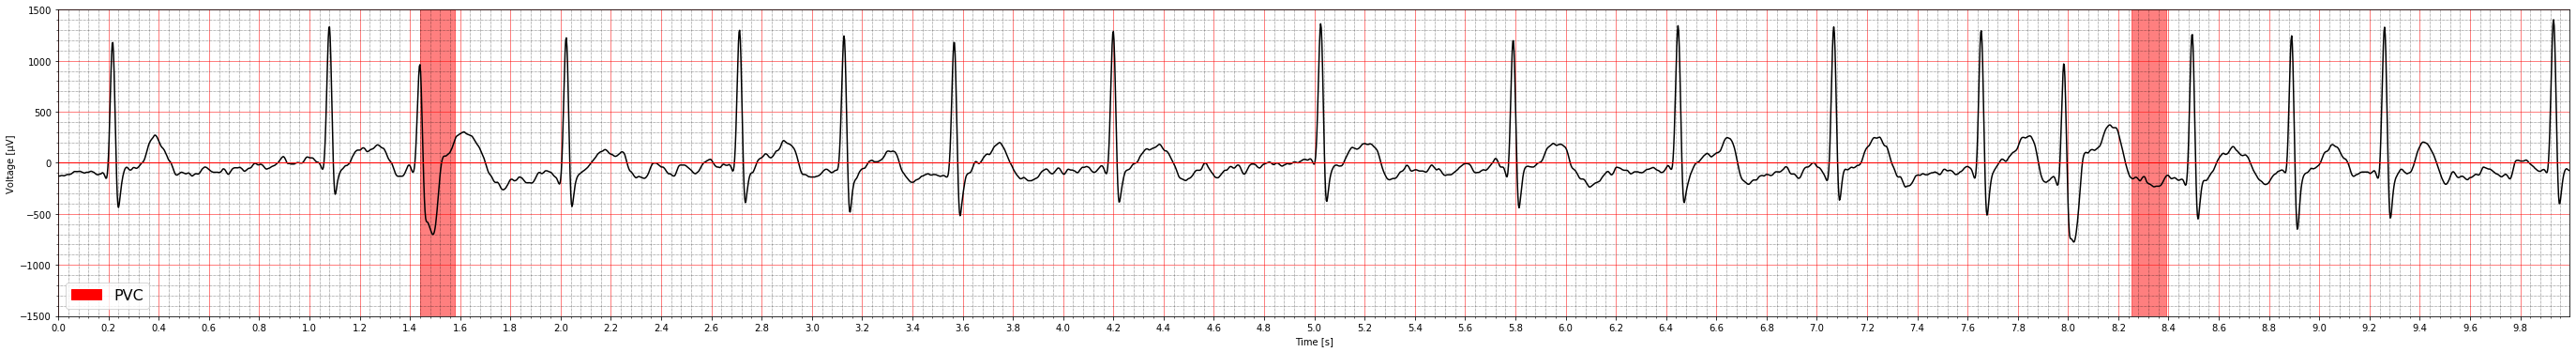
\includegraphics[width=\textwidth,keepaspectratio]{images/CPSC2020_A02_AF1.png}
\end{figure}
\end{block}

\uncover<6->{\bfseries 心律异常种类可高达上百种,且有可解释性的需求}

\end{frame}

%------------------------------------------------
% Page 15

\begin{frame}
\frametitle{深度学习应用于生理信号处理}

\begin{columns}

\begin{column}{0.67\textwidth}
\begin{block}{Motivation}<1->

\uncover<2->{{\large Stanford ML Group}}
\vspace{1em}

\uncover<3->{\textit{``Cardiologist-level arrhythmia detection and classification in ambulatory electrocardiograms using a deep neural network''}}
\vspace{1em}

\uncover<4->{{\large Nature Medicine}, volume 25, pages 65–69 (2019)}

\end{block}

\vspace{0.6em}

\uncover<3->{\raggedleft 模型结构:modified resnet34 $\rightarrow$}

\end{column}

\begin{column}{0.3\textwidth}
\uncover<3->{
\begin{figure}
    \centering
    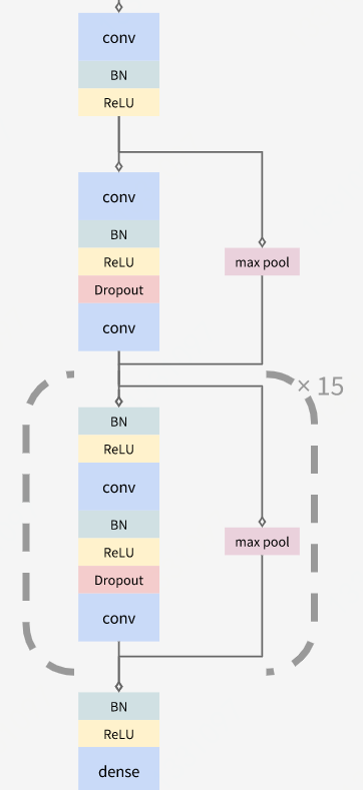
\includegraphics[width=\textwidth,keepaspectratio]{images/stanford_resnet34.png}
\end{figure}}
\end{column}

\end{columns}

\end{frame}

%------------------------------------------------
% Page 7

\begin{frame}
\frametitle{深度学习应用于生理信号处理}

\uncover<1->{
\begin{figure}
\centering
\begin{tikzpicture}[remember picture]
\node [rectangle] (resnet34) {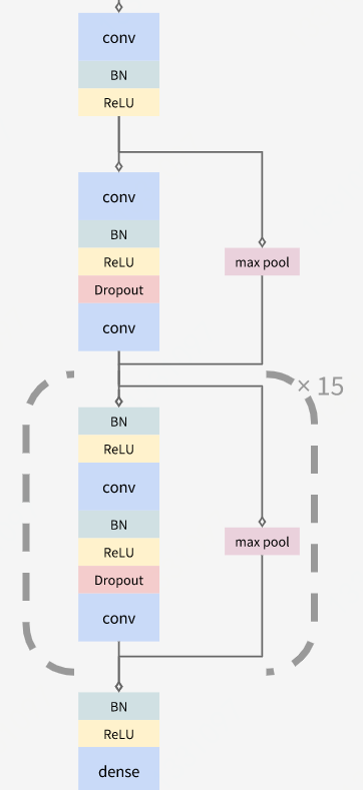
\includegraphics[width=0.25\textwidth,keepaspectratio]{images/stanford_resnet34.png}};
\node [rectangle, below left = 0.7cm and 1.4cm of resnet34.north] (cnn) {\footnotesize CNN};
\node [rectangle, below = 0.3cm of cnn.south] (resnet34_text) {\footnotesize resnet34};
\node [rectangle, below right = 0.7cm and 1.25cm of resnet34.north] (plus1) {
\includegraphics[width=0.05\textwidth,keepaspectratio]{images/gray_plus.png}};
\node [rectangle, below right = 0.7cm and 2.1cm of resnet34.north] (rnn) {\footnotesize RNN};
\node [rectangle, below = 0.7cm of rnn.south] (lstm) {{\tiny 双向LSTM}};
\node [rectangle, below = 0.5cm of lstm.south] (linear) {{\tiny Linear}};
\node [rectangle, below = 0.5cm of linear.south] (crf) {{\tiny \color{red} CRF}};
\node [rectangle, below right = 0.7cm and 3.15cm of resnet34.north] (plus2) {
\includegraphics[width=0.05\textwidth,keepaspectratio]{images/gray_plus.png}};
\node [rectangle, below right = 0.7cm and 3.9cm of resnet34.north] (pr) {\footnotesize ``伪''PR间期后处理};
\node [rectangle, below = 1.1cm of pr.north] (pr_dist) {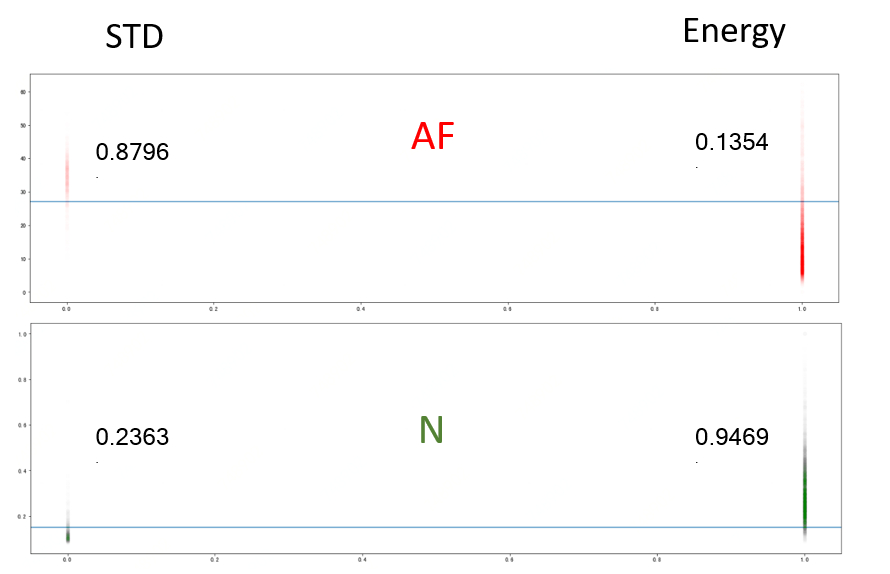
\includegraphics[width=0.37\textwidth,keepaspectratio]{images/pseudo_pr_dist_cinc2017.png}};

\path[->] ([yshift = -0.05cm]lstm.south) edge ([yshift = 0.05cm]linear.north);
\path[->] ([yshift = -0.05cm]linear.south) edge ([yshift = 0.05cm]crf.north);
\end{tikzpicture}
\end{figure}
}

\uncover<2->{
\footnotesize 其他一些{\color{red}数据增强}{\color{zkblue} trick: random masking QRS complexes}
}

\end{frame}

%------------------------------------------------
% Page 8

\begin{frame}
\frametitle{深度学习应用于生理信号处理}

\begin{itemize}
\item<1-> CinC2020: \textit{\scriptsize Classification of 12-lead ECGs: the PhysioNet - Computing in Cardiology Challenge 2020}
\item<1-> {\color{red} CPSC2020}: \textit{\scriptsize Searching for Premature Ventricular Contraction and Supraventricular Premature Beat from Long-term ECGs: The 3rd China Physiological Signal Challenge 2020}

\uncover<2->{
\begin{figure}
\centering
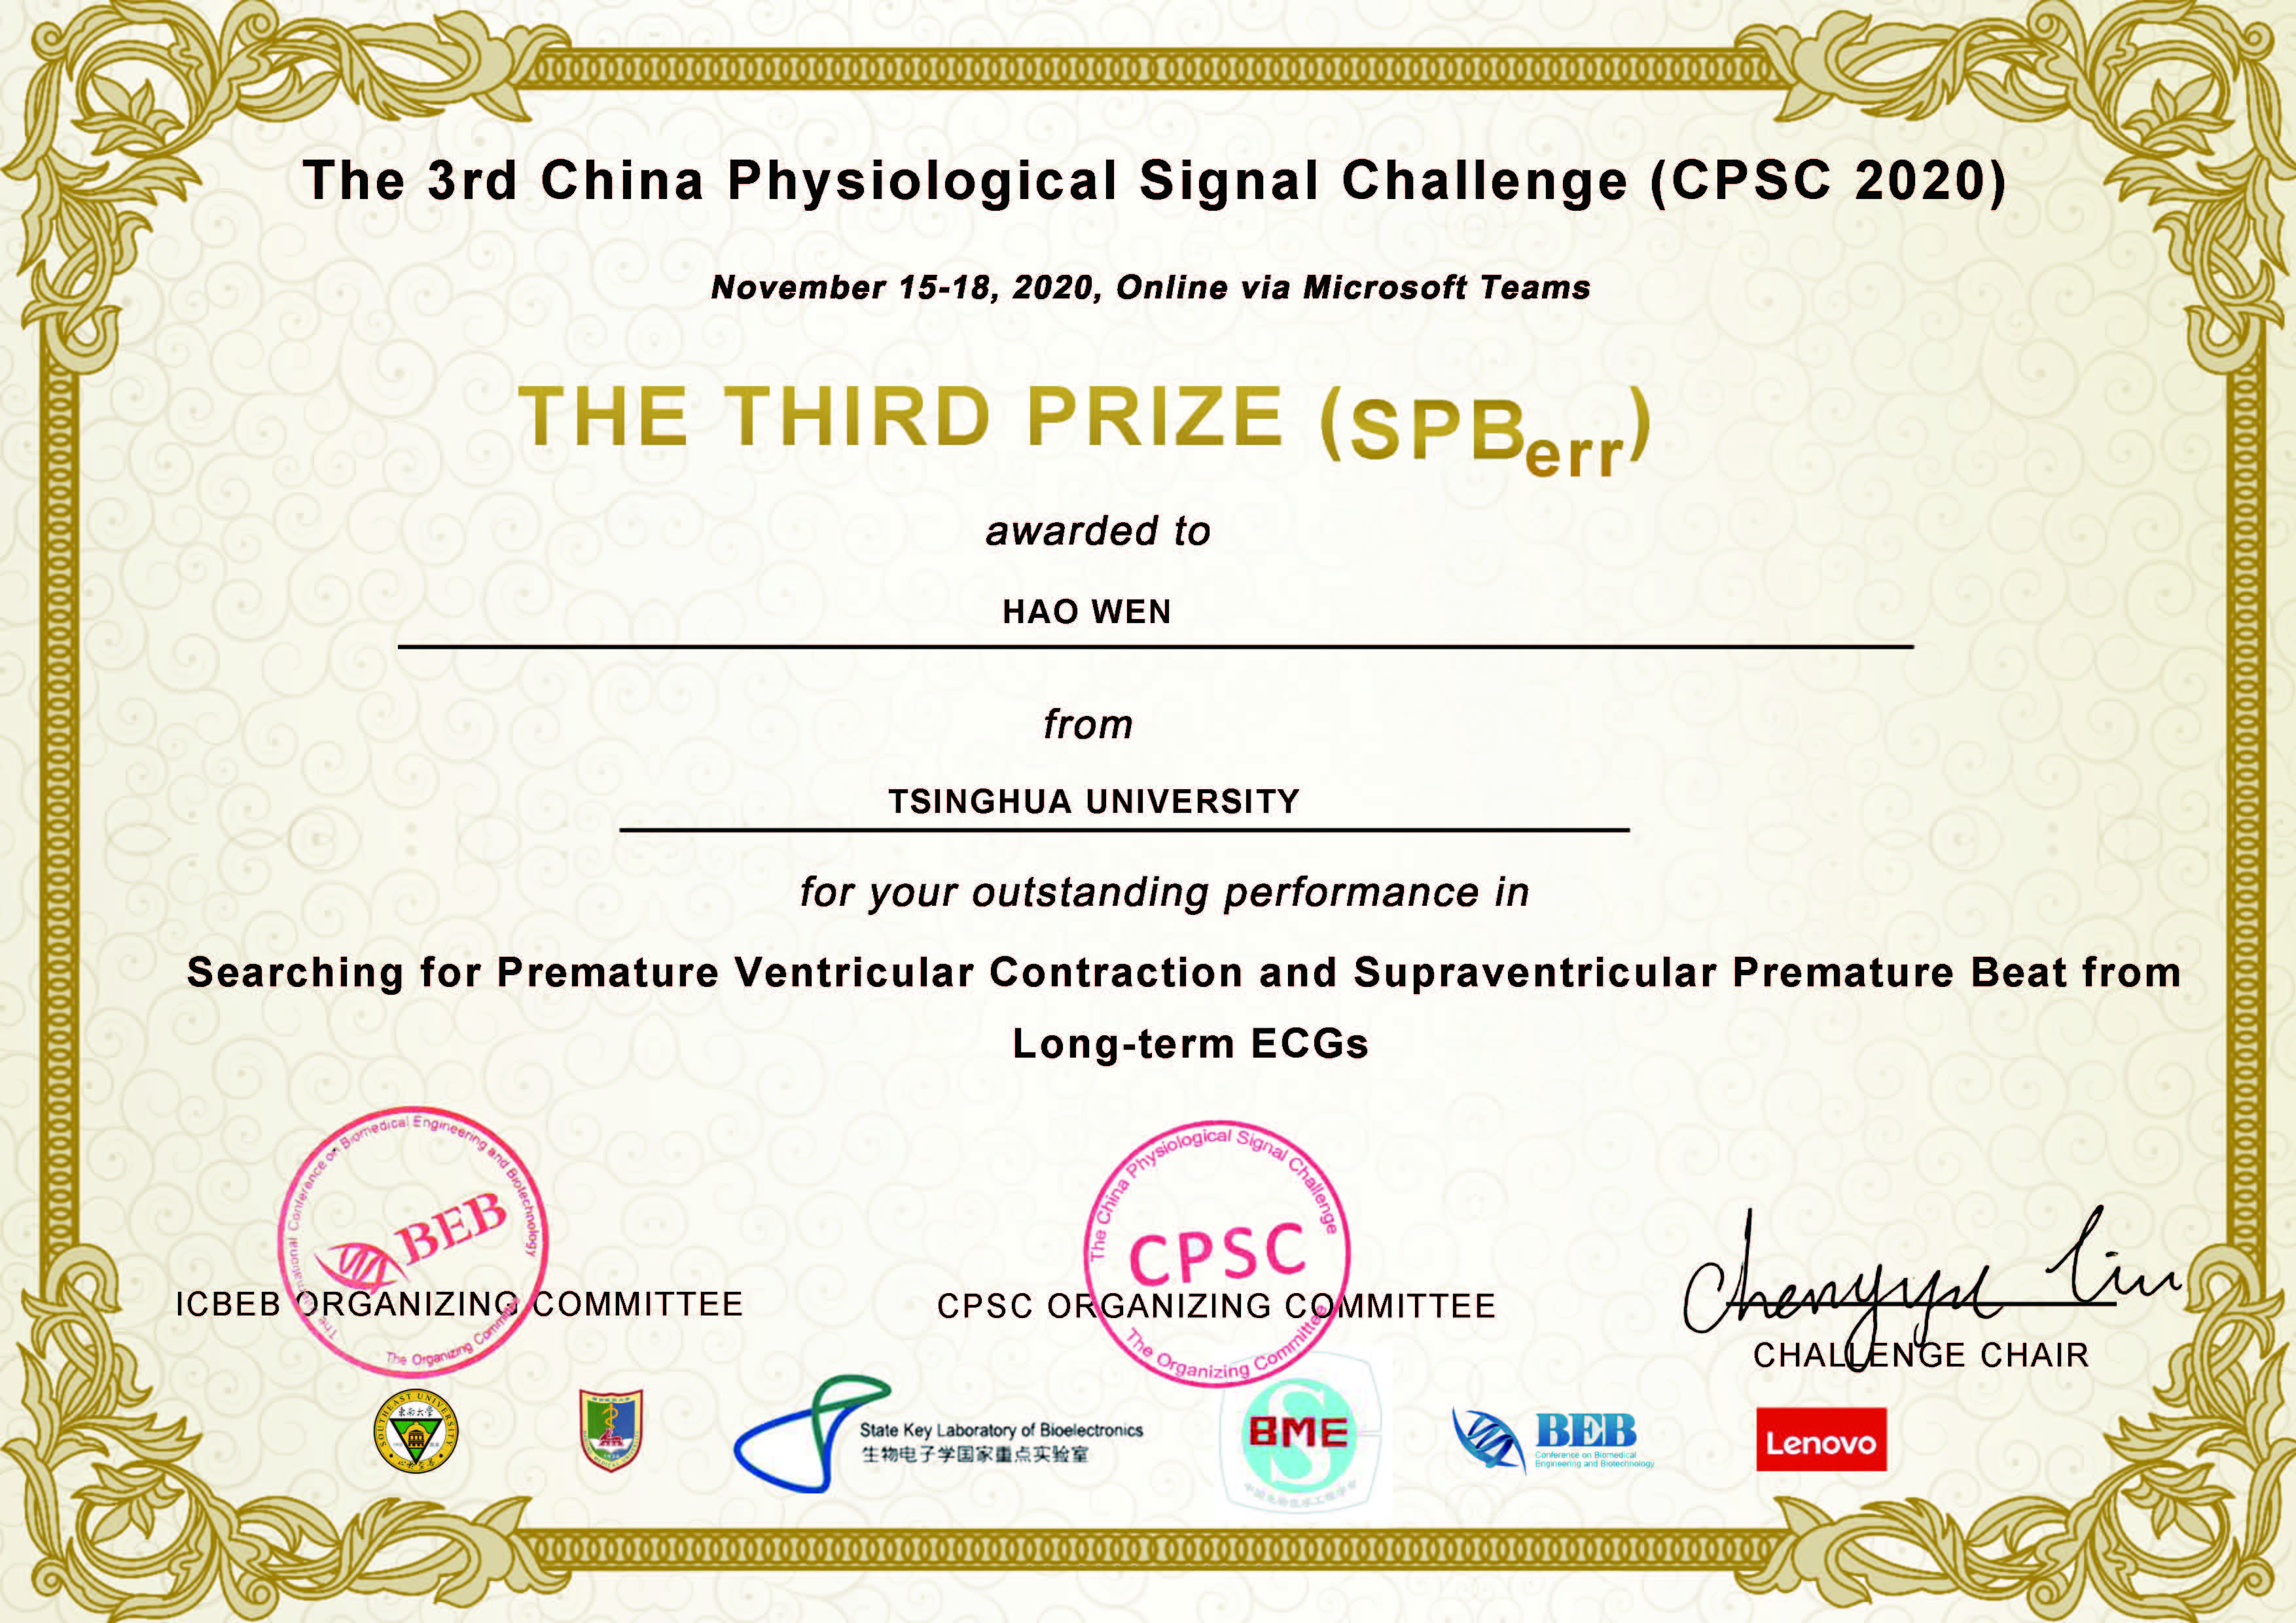
\includegraphics[width=0.37\textwidth,keepaspectratio]{images/CPSC2020_SPBerr_3rd.jpg}
\end{figure}
}

\item<1-> CinC2021 {\scriptsize (ongoing)}: \textit{\scriptsize Will Two Do? Varying Dimensions in Electrocardiography: The PhysioNet/Computing in Cardiology Challenge 2021}
\item<1-> CPSC2021 {\scriptsize (ongoing)}: \textit{\scriptsize Paroxysmal Atrial Fibrillation Events Detection from Dynamic ECG Recordings: The 4th China Physiological Signal Challenge 2021}
\end{itemize}

\end{frame}

%------------------------------------------------
% Page 10

\begin{frame}
\frametitle{深度学习应用于生理信号处理}

CinC2021一次试验(的metrics)的例子:

\begin{figure}
\centering
\begin{tikzpicture}[remember picture]
    \coordinate (slide_center) at (0,0);
    \node[above=2cm of slide_center] (eg_train_cinc2021) {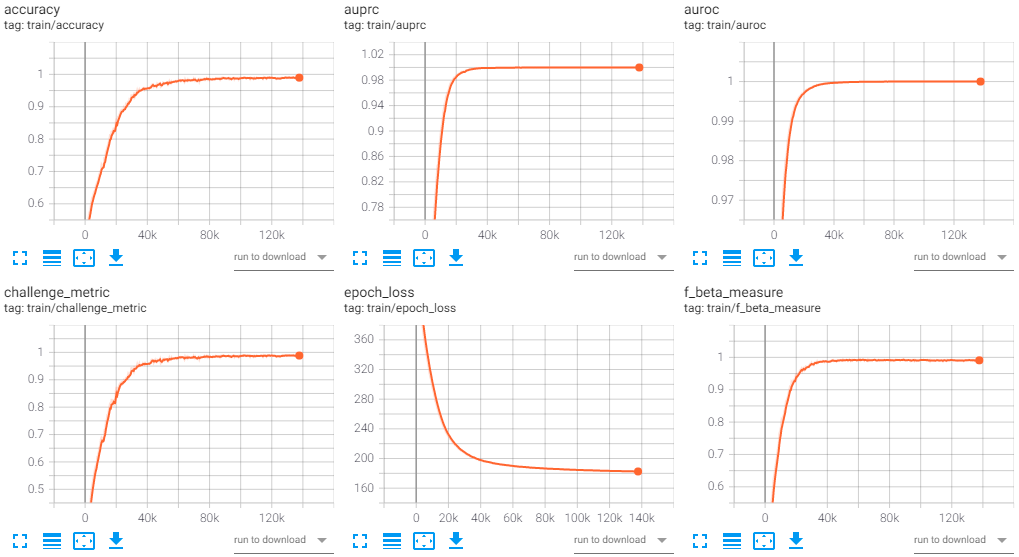
\includegraphics[width=0.6\textwidth,keepaspectratio]{images/eg_train_cinc2021.png}};
    \node[left=1cm of eg_train_cinc2021.west] () {train};
    \node[below=0.2cm of eg_train_cinc2021.south] (eg_test_cinc2021) {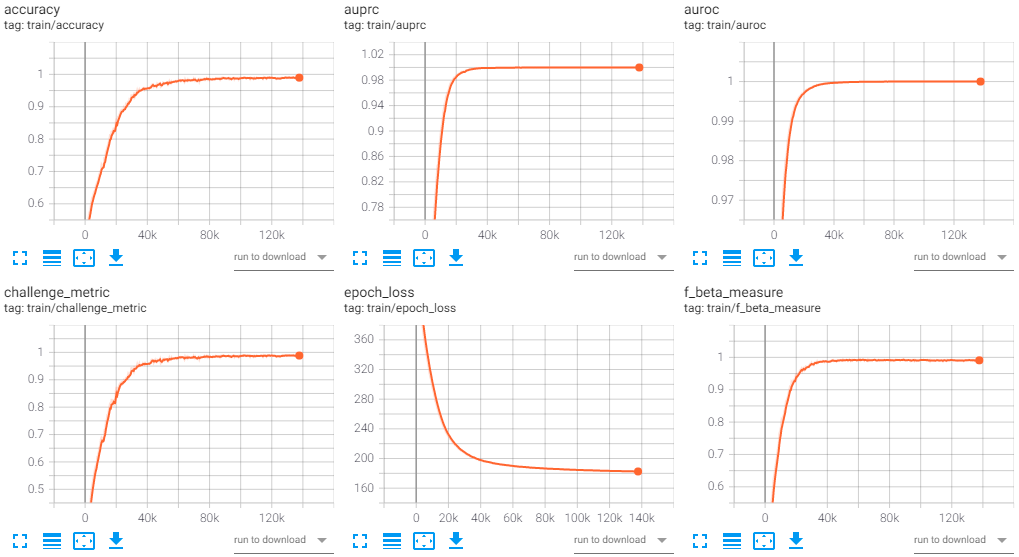
\includegraphics[width=0.6\textwidth,keepaspectratio]{images/eg_test_cinc2021.png}};
    \node[left=1cm of eg_test_cinc2021.west] () {test};
\end{tikzpicture}
\end{figure}

\end{frame}

%------------------------------------------------
% Page 10

\begin{frame}
\frametitle{深度学习应用于生理信号处理}

一些主要的GitHub仓库

\vspace{1.2em}

\begin{itemize}
\item \href{https://github.com/wenh06/cinc2020}{https://github.com/wenh06/cinc2020}
\vspace{0.8em}
\item \href{https://github.com/wenh06/cpsc2020}{https://github.com/wenh06/cpsc2020}
\vspace{0.8em}
\item \href{https://github.com/wenh06/torch_ecg}{https://github.com/wenh06/torch\_ecg}
\vspace{0.8em}
\item \href{https://github.com/wenh06/cinc2021}{https://github.com/wenh06/cinc2021} (private)
\vspace{0.8em}
\item \href{https://github.com/wenh06/cpsc2021}{https://github.com/wenh06/cpsc2021} (private)
\end{itemize}

\end{frame}

%------------------------------------------------

\section[NLP]{Natural Language Processing}

%------------------------------------------------
% Page 15

\begin{frame}
\frametitle{PharmCoo合理用药系统}

\begin{figure}
\centering
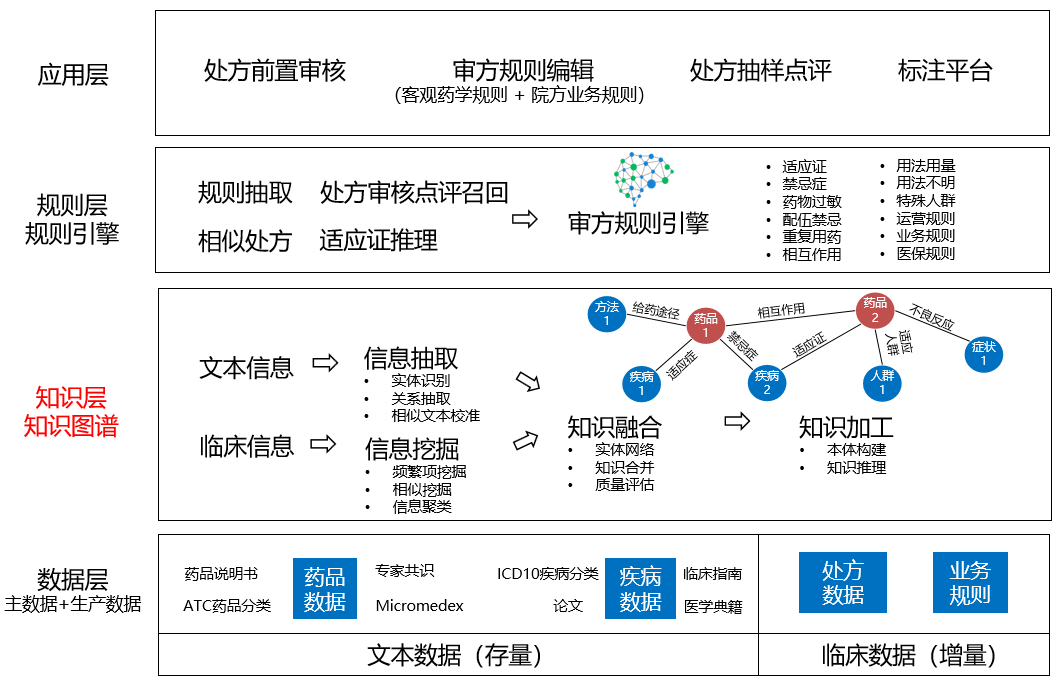
\includegraphics[width=0.98\textwidth,keepaspectratio]{images/pharmcoo.png}
\end{figure}

\end{frame}

%------------------------------------------------
% Page 15

\begin{frame}
\frametitle{药学知识图谱知识抽取整体架构}

\begin{figure}
\centering
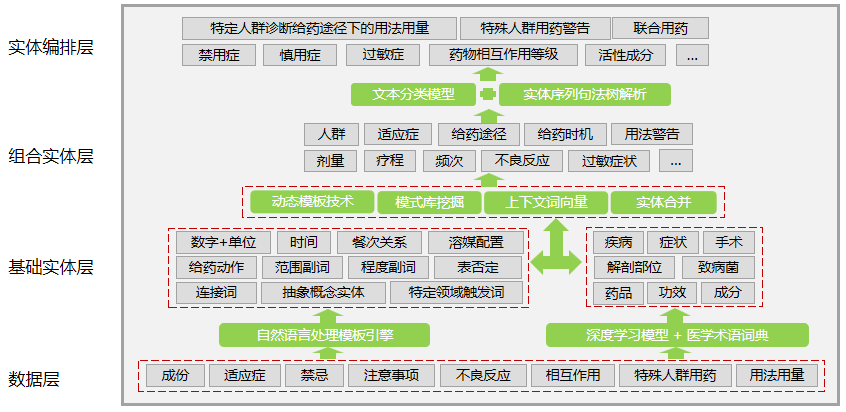
\includegraphics[width=0.98\textwidth,keepaspectratio]{images/med_knowledge_graph.png}
\end{figure}

\end{frame}

%------------------------------------------------
% Page 15

\begin{frame}
\frametitle{知识抽取的例子}

\begin{figure}
\centering
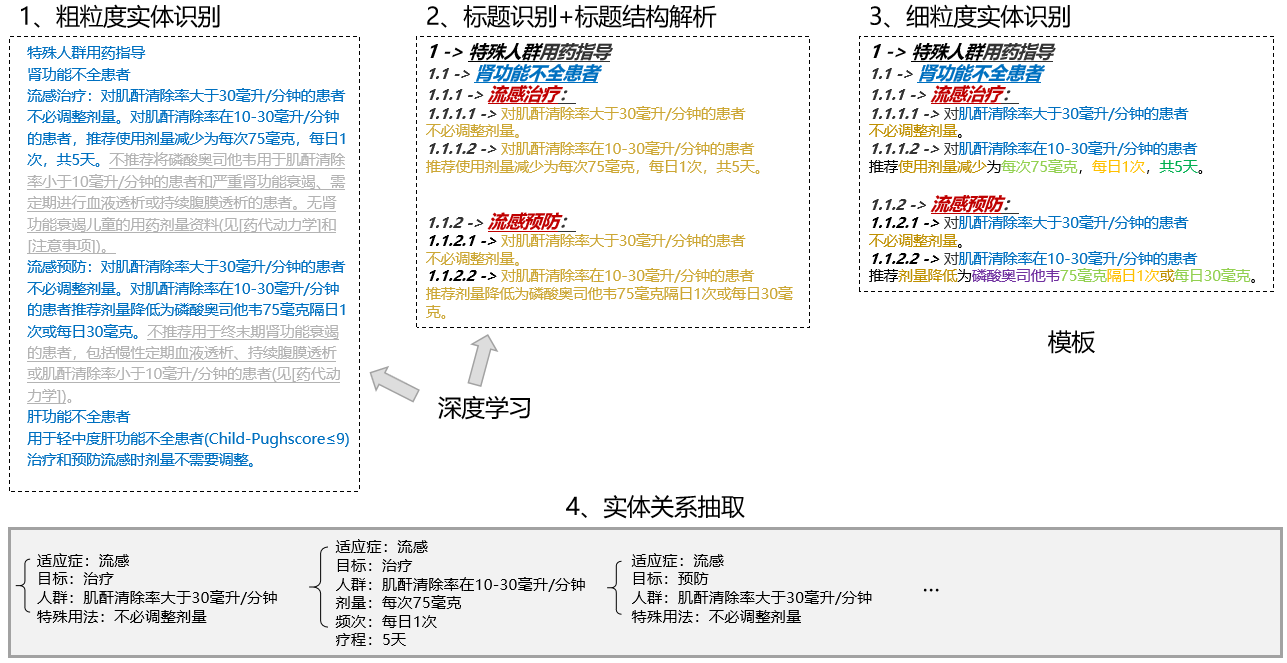
\includegraphics[width=0.98\textwidth,keepaspectratio]{images/di_parsing.png}
\end{figure}

\pause
\vspace{0.5em}

\href{https://github.com/wenh06/med_nlp}{https://github.com/wenh06/med\_nlp} (private)

\end{frame}

%------------------------------------------------
% Page 15

\begin{frame}
\frametitle{实际使用}

PharmCoo合理用药系统目前已经在以下的场景投入实际的使用:

\vspace{0.8em}

\begin{itemize}
    \item 京东健康互联网医院前置审方
    \item 海淀区多家医院(海淀卫健委)前置审方
\end{itemize}

\pause
\vspace{1em}

at the cost of:

\begin{figure}
\centering
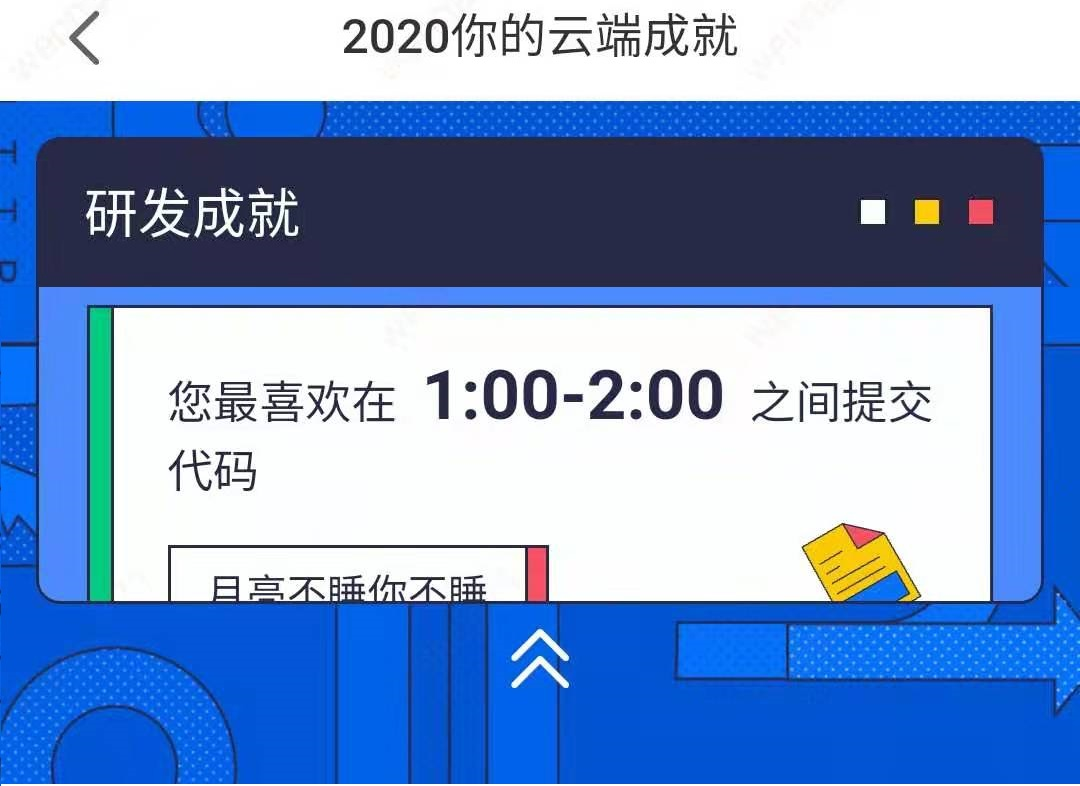
\includegraphics[width=0.43\textwidth,keepaspectratio]{images/jd_coding_stats.jpg}
\end{figure}

\end{frame}

%------------------------------------------------
% Page 15

\begin{frame}
\frametitle{尚存痛点}

\begin{itemize}
    \item 数据共享问题
    \vspace{0.6em}
    \item {\color{green}高效}{\color{pink}准确}的{\color{red}细粒度}数据标注
    \vspace{0.6em}
    \item 中医审方
    \vspace{0.6em}
    \item etc.
\end{itemize}

\end{frame}

%------------------------------------------------

\section[CGM]{Continuous Glucose Monitoring}

%------------------------------------------------
% Page 15

\begin{frame}
\frametitle{连续血糖 --- 生理模型}

\begin{columns}

\begin{column}{0.5\textwidth}
{\scriptsize
\begin{itemize}
    \item 胃肠
    \begin{align*}
    \dfrac{d g^{sto\_u}(t)}{dt} = & -k_{21} \cdot g^{sto\_u}(t) \\
    \dfrac{d g^{sto\_d}(t)}{dt} = & -k_{e} \cdot g^{sto\_d}(t) \\ 
    & + k_{21} \cdot g^{sto\_u}(t) \\
    \dfrac{\partial g(z,t)}{\partial t} = & -\overline{u}\dfrac{\partial g(z,t)}{\partial z} - \overline{K}\cdot g(z,t)
    \end{align*}
    \item 血糖
    \begin{align*}
    \dfrac{dG^{pl}}{dt} = & \~ g^{liv}(t) + g^{gut}(t) \\
    & - g^{non-it}(t) - g^{it}(t) - g^{ren}(t)
    \end{align*}
    \item 胰岛素
    $$\dfrac{dI^{pl}}{dt} = i^{pnc}(t) - i^{liv}(t) - i^{if}(t)$$
\end{itemize}
}
\end{column}

\begin{column}{0.5\textwidth}
\begin{figure}
\centering
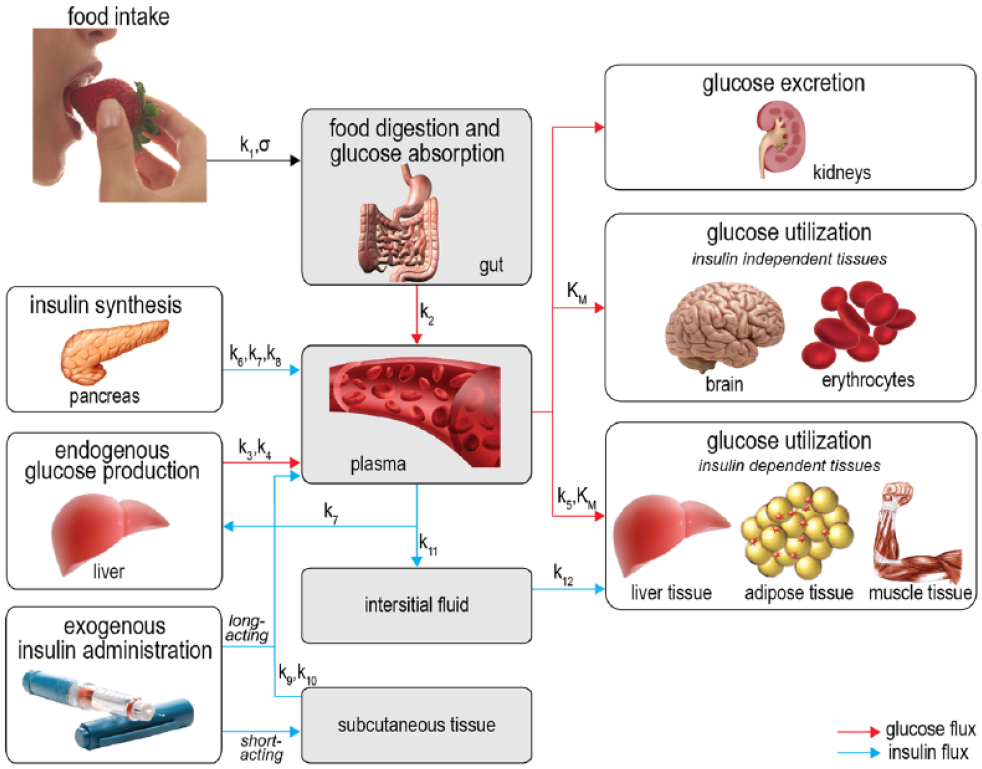
\includegraphics[width=1\textwidth,keepaspectratio]{images/bg_model.png}
\end{figure}
\end{column}

\end{columns}


\end{frame}

%------------------------------------------------
% Page 15

\begin{frame}
\frametitle{血糖 --- 生理模型}

用途:预测餐后血糖,评估运动对血糖影响

\vspace{1em}

\uncover<2->{
一些问题:
}
\begin{itemize}
    \item<3-> 实际使用的时候,胰岛素浓度没有方便途径采集,导致整个模型是structural non-identifiable的(是一个病态的问题,解局部不唯一)。
    \item<4-> 即使固定一些未知量,模型参数拟合计算慢(scipy.optimize Nelder-Mead),但这与precision health本意相违背了。
\end{itemize}

\end{frame}

%------------------------------------------------
% Page 15

\begin{frame}
\frametitle{夜间低血糖预测模型}

\uncover<2->{
方法(专利):从连续血糖数据提取一系列特征
}
\vspace{0.6em}

\uncover<3->{
模型:二分类XGBoost
}
\vspace{0.6em}

\uncover<4->{
该模型在生产环境中使用,对于二型糖尿病人的夜间低血糖事件的预警非常有效。
}
\vspace{1em}

\uncover<5->{
\begin{remark_cn}
XGBoost带来的一个问题是,不太好做incremental learning. 
\begin{quote}
    ``the tree construction algorithm works differently than SGD. In a sense that SGD can be incremental, while tree construction algorithm is in nature batch, you want to see all the data before you decide which one is the best split.'' \hfill -- Tianqi Chen
\end{quote}
\end{remark_cn}
}

\end{frame}

%------------------------------------------------

\section[Misc]{Miscellaneous}

%------------------------------------------------
% Page 15

\begin{frame}
\frametitle{Miscellaneous}

\begin{itemize}
    \item<2-> 中医望诊系统(面诊、舌诊、手诊) --- 图像
    \item<3-> 饮食营养分析 --- 图像
    \begin{columns}
    \begin{column}{0.45\textwidth}
    \begin{figure}
        \centering
        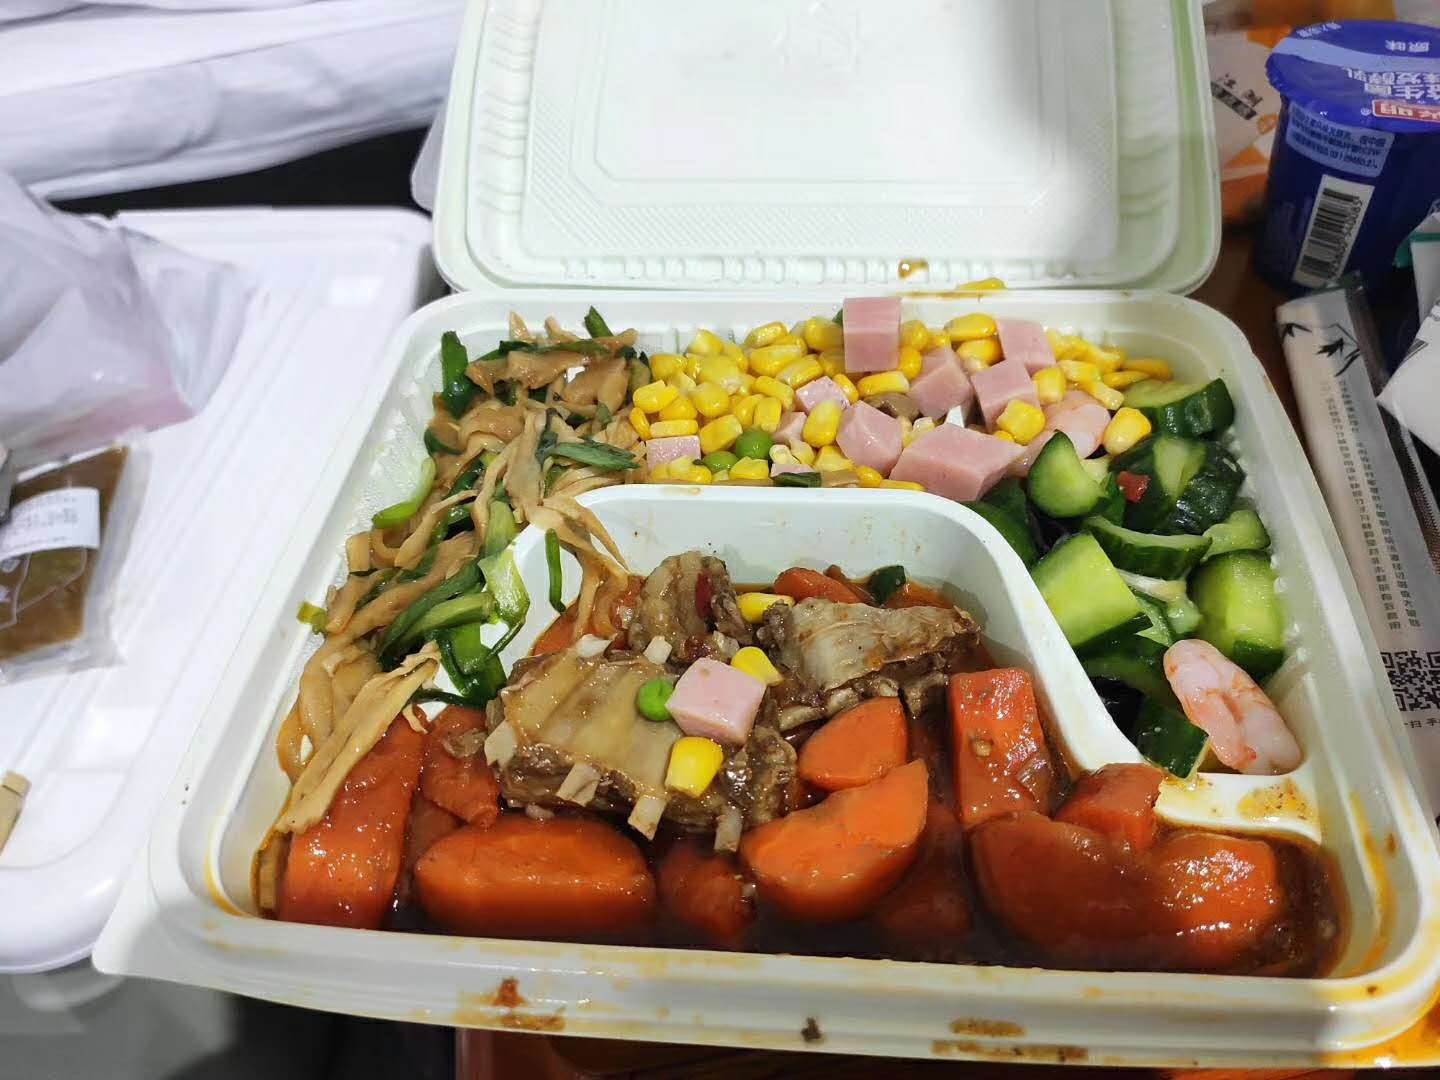
\includegraphics[width=1\textwidth,keepaspectratio]{images/diet_img.jpg}
    \end{figure}
    \end{column}
    \begin{column}{0.24\textwidth}
    \begin{figure}
        \centering
        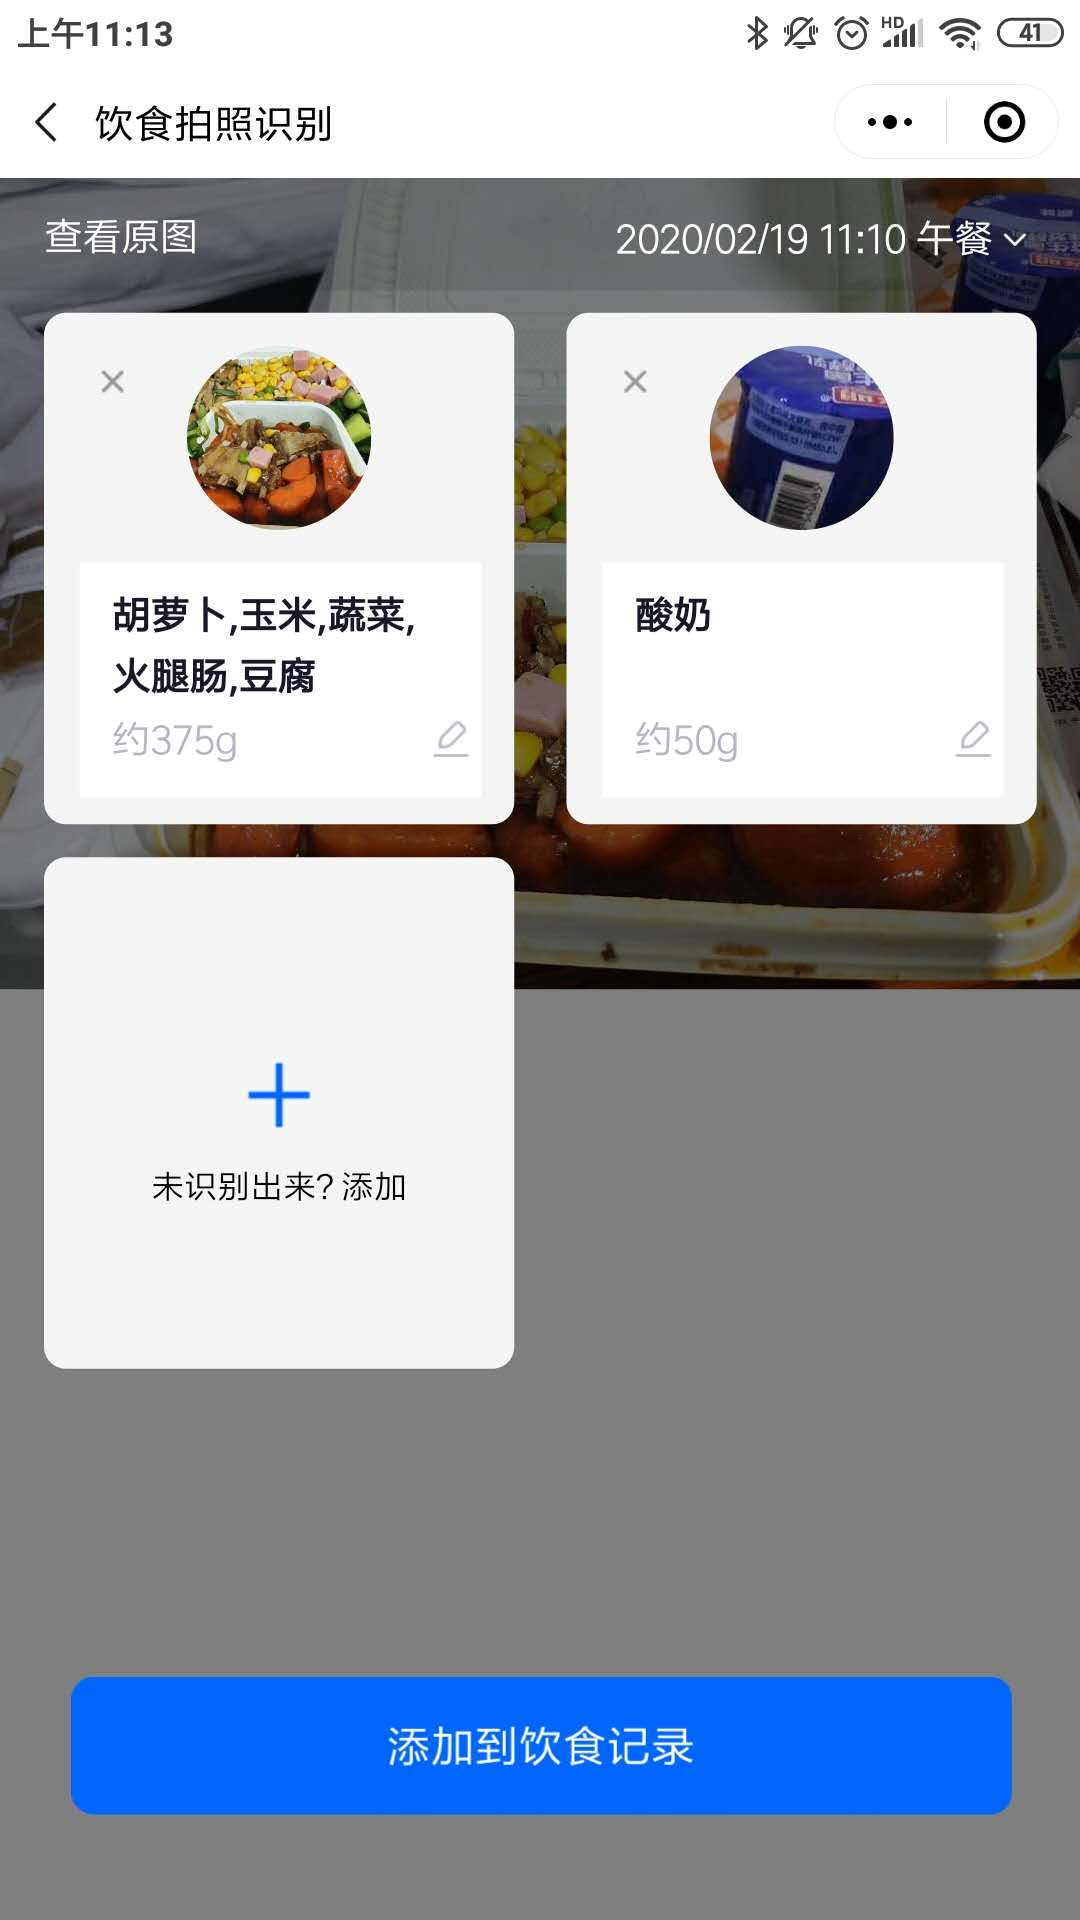
\includegraphics[width=1\textwidth,keepaspectratio]{images/diet_ann_res.jpg}
    \end{figure}
    \end{column}
    \end{columns}
    \item<4-> 多模态(actigraph, ECG, PPG, audio, ...)睡眠分析(sleep stage, sleep apnea, ...)
    \item<5-> etc. (\href{https://github.com/wenh06/utils}{https://github.com/wenh06/utils})
\end{itemize}

\end{frame}


%------------------------------------------------

\begin{frame}

\Huge{\centerline{\bfseries The End}}

\vspace{0.5em}

\Huge{\centerline{\phantom{a}\bfseries 谢谢!}}

\end{frame}

%------------------------------------------------

\end{document}
